\section{Experimentos e resultados} 

Dado que o sistema de planejamento é geral, foram feitos dois experimentos, para o mundo dos blocos e para o mundo dos satélites. Os dados de entrada são os proporcionados na página no curso (ver \cite{LabIA15}).

\subsection{Experimentos com mundo dos blocos}
\label{subsec:expblocos}
	
		\begin{figure}[H]
			\centering
			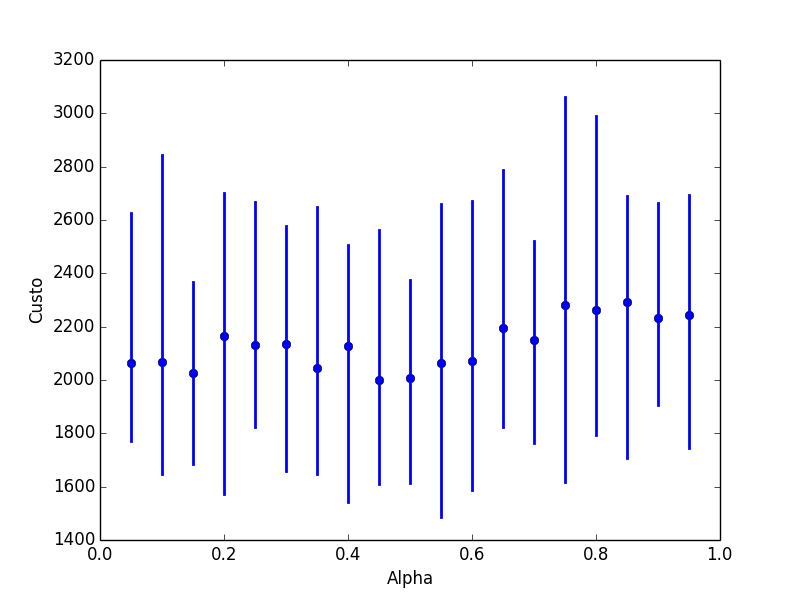
\includegraphics[height=8cm]{images/cost_distance_alpha}
			\caption{Custos com distancia}
			\label{fig:costdistancealpha}
		\end{figure}
		
		\begin{figure}[H]
			\centering
			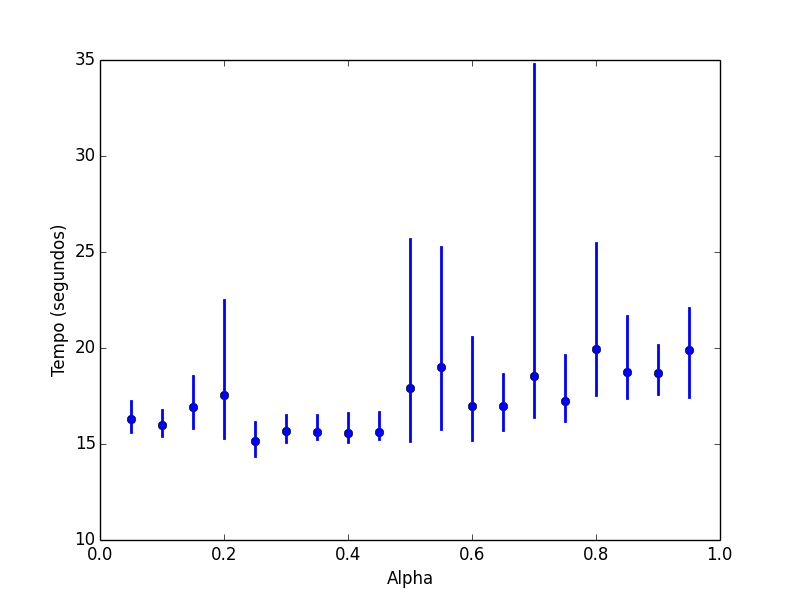
\includegraphics[height=8cm]{images/time_distance_alpha}
			\caption{Tempo com distancia}
			\label{fig:timedistancealpha}
		\end{figure}

 \subsection{Experimentos com mundo dos satelites}
\label{subsec:expsatelites}